
The rocket, entitled RORO I, is a 8 feet (2.45 meters) rocket propelled by a M-class solid motor. The main requirements of the rocket are presented in Table \ref{table:se_topLevelR}.

\begin{table}[h!]
\centering
\begin{tabular}{|p{0.9\columnwidth}|}
\hline
    The rocket shall achieve an apogee of 10,000 ft (3048 meters).  \\ \hline
    The rocket shall have a static margin between 1 and 2 body-calibers \\ \hline
    The rocket shall carry a COTS barometric pressure altimeter with on-board storage as primary data source for altitude reporting.  \\ \hline
    The launch vehicle shall follow a "dual-event" recovery \\ \hline
    The rocket shall carry a minimum mass of 8.8 lb (4 kg) of payload. \\ \hline
    The rocket shall eject its nosecone at apogee. \\ \hline
    The rocket shall release a glider from the payload section at 10 seconds after apogee. \\ \hline

\end{tabular}
\caption{Top Level Requirements for the rocket}
\label{table:se_topLevelR}
\end{table}


\subsection{Design and Manufacturing}


The rocket is divided into 3 main sub-assemblies (Figure \ref{f:rocket_adnoted}:
\begin{enumerate}
    \item The nosecone - carrying avionics and an ejection system
    \item Upper Body - carrying the payload, the parachutes and the recovery electronics
    \item The Lower Body - containing logging avionics and the motor
\end{enumerate}
The concept of the rocket was well-thought to be easy to integrate and robust, considering the time constrains. The rocket separated in the middle, between the upper and lower body. This approach is very common in High Power Rocketry (HPR) and is considered a less risky approach.

\begin{figure}[h!]
\centering
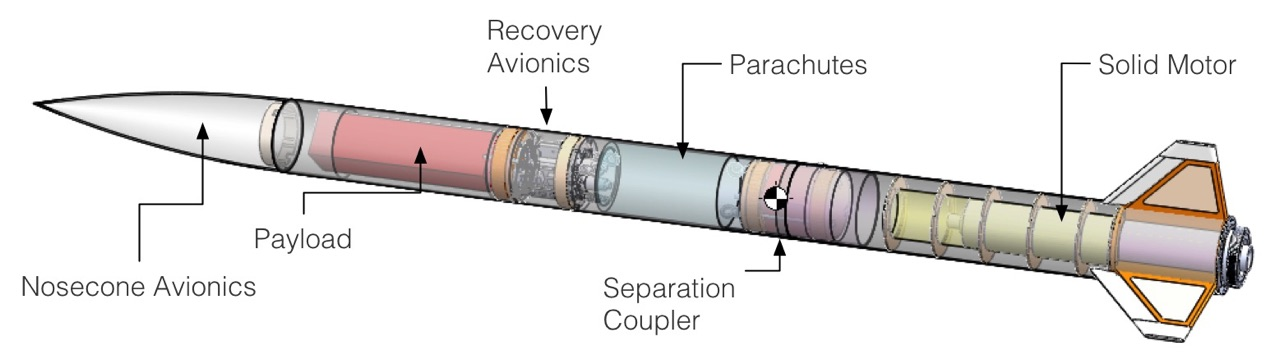
\includegraphics[width=0.5\textwidth]{img/rocket_sw_annotated.jpg}
\caption{The rocket with its main components}
\label{f:rocket_adnoted}
\end{figure}

The length as well as the diameter of the rocket were chosen in such a way to accommodate the payload which had a dimension constraint imposed by the competition (needed to be Cubesat standard).

Two important factors are important in a rocket: the dynamic stability and the static stability.


Now, the manufacturing of each part of the rocket is discussed.



\paragraph{Structure}
\hfill \break
The main body of the rocket is a COTS phenolic tube, reinforced with two layers of 245 g/m$^2$ twill weaved carbon fiber. The reinforcement rational was determined using FEA (Finite Element Analysis), and tested during two rocket flights.
The structure contains also a coupler tube, that is made out of phenolic tube reinforced inside again with two 245 g/m$^2$ layers carbon fiber.
The rocket has two structural bulkheads, one in the lower body and one in the upper body to which the parachute cords are attached. The bulkheads were made out of two 15mm plywood plates reinforced with 4 layers of 245 g/m$^2$ carbon fibre on each side.  The bulkheads are the structurally critical elements as they transfer loads from the rocket body to the subsystems. They need to withstand both the accelerations from the launch and the parachute opening shock. 
The two bulkheads are subject to a peak load of 10kN from the parachute opening shock. An FEM analysis taking into account the  ECSS-E-HB-32-21A revealed that an additional reinforcement of the bulkheads with carbon fibre is required to sustain the loads. The analysis of the bonding to the rocket body reveals sufficient strength to sustain the opening shock.


\paragraph{Fins}
\hfill \break
    The fins were sized for 1.1 calibers static stability %Reference to static/dynamic stability
    The fins were manufactured out of wood and carbon fiber, as it can be seen in Figure \ref{f:fins}. Firstly, the wood was cut at CNC (Figure \ref{f:fins} a). The inside of the fins was made out of balsa wood (Figure \ref{f:fins} b), in order to decrease the weight for higher resonance frequencies. Afterwards, on each side of each fin, 3 layers [span, chord, span] of 140 g/m$^2$ unidirectional carbon fiber were applied, to increase stiffness (Figure \ref{f:fins} c). The fins were attached to the motor tube using high temperature epoxy, reinforced with carbon fiber.
    \begin{figure}[h!]
        \centering
        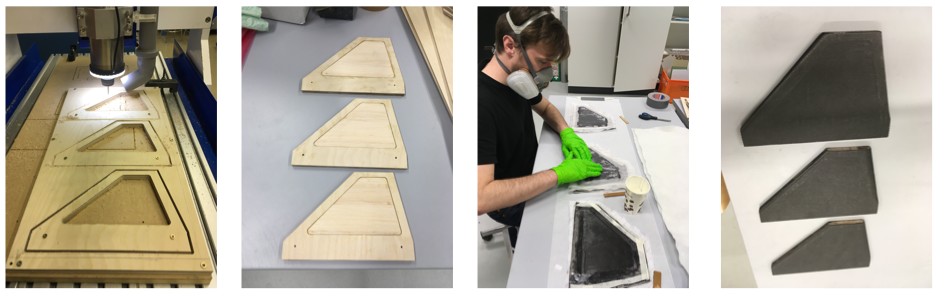
\includegraphics[width=0.5\textwidth]{img/fins.png}
        \caption{a) Wood at CNC b) Final wood-made fins c) Carbon fiber manufacturing d) Final version of the fins.}
        \label{f:fins}
    \end{figure}


\paragraph{Motor tube}
\hfill \break
The motor tube consists of a Commercial-Off-The-Shelf phenolic tube. The fins were glued with 3M DP760 high-temperature epoxy to the motor tube. The tube was centered to the outer rocket body tube by six 4mm plywood centering rings distributed in equally along the motor tube.
In front of the fins, there is a 12mm CNC-cut plywood ring from which 12 M3 threaded rods connect to the thrust plate. These help holding the motor inside the rocket body during parachute opening shock.
The entire assembly can be seen in Figure \ref{f:reinforcement} c. The fins were fixed to the outer structure using ribbons of carbon fiber both on the inside and the outside of the tube, as it can be seen in Figure \ref{f:reinforcement} a,b.

  \begin{figure}[h!]
\centering
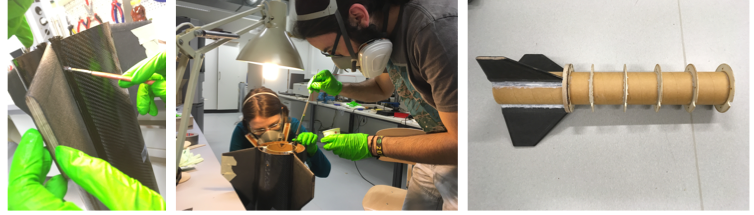
\includegraphics[width=0.5\textwidth]{img/fins_glue.png}
\caption{a, b) Reinforcement of the fins c)Motor tube assembly, with fins and centering rings}
\label{f:reinforcement}
\end{figure}


\paragraph{Motor case}
\hfill \break
The motor case, which is a RMS-98/7680 from Aerotech is held by a 98mm retainer from Aeropack on a custom made laser-cut aluminum thrust plate. The thrust-plate pushes directly on the fins which go through the body tube to the motor tube. The thrust-plate is used to attach the motor and to distribute the loads when parachute opens.
 The retainer \& thrust-plate assembly can be seen in Figure \ref{f:motor_retainer_2}.
\begin{figure}[h!]
        \centering
        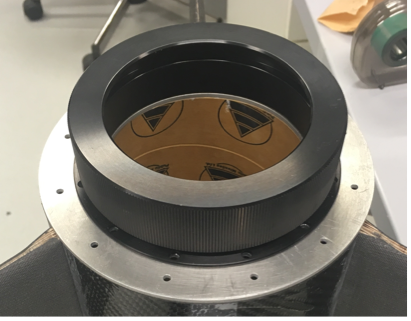
\includegraphics[width=0.3\textwidth]{img/motor_retainer.png}
        \caption{Motor Retainer and the Aluminum plate}
        \label{f:motor_retainer_2}
    \end{figure}


\paragraph{Payload}
\hfill \break
In the lower body of the rocket, there is 1U of payload consisting of 4kg of tungsten and a board with sensors used to track the lower body motion and shocks, referred to as the Logging Electronics. A Gopro and a PCB cameras are also placed to film the parachute deployment and the outside.
The Active Payload bay, placed in the Upper Body, consists of a 4U plywood box reinforced with glass fibre to withstand the loads. Inside the 4U wood box, a glider is mounted on a rail. Shortly after apogee, the glider will be ejected from the rocket using a spring. A more detailed description of the glider will be detailed in the second part of the article.



\subsection{Recovery}
The Recovery Subsystem implements a dual-event recovery CONOPS with an initial deployment event at apogee and a main deployment event at 457m (1500ft) AGL. Figure \ref{f:recovery_conops} illustrates the recovery CONOPS.
\begin{figure}[h!]
 	\centering
        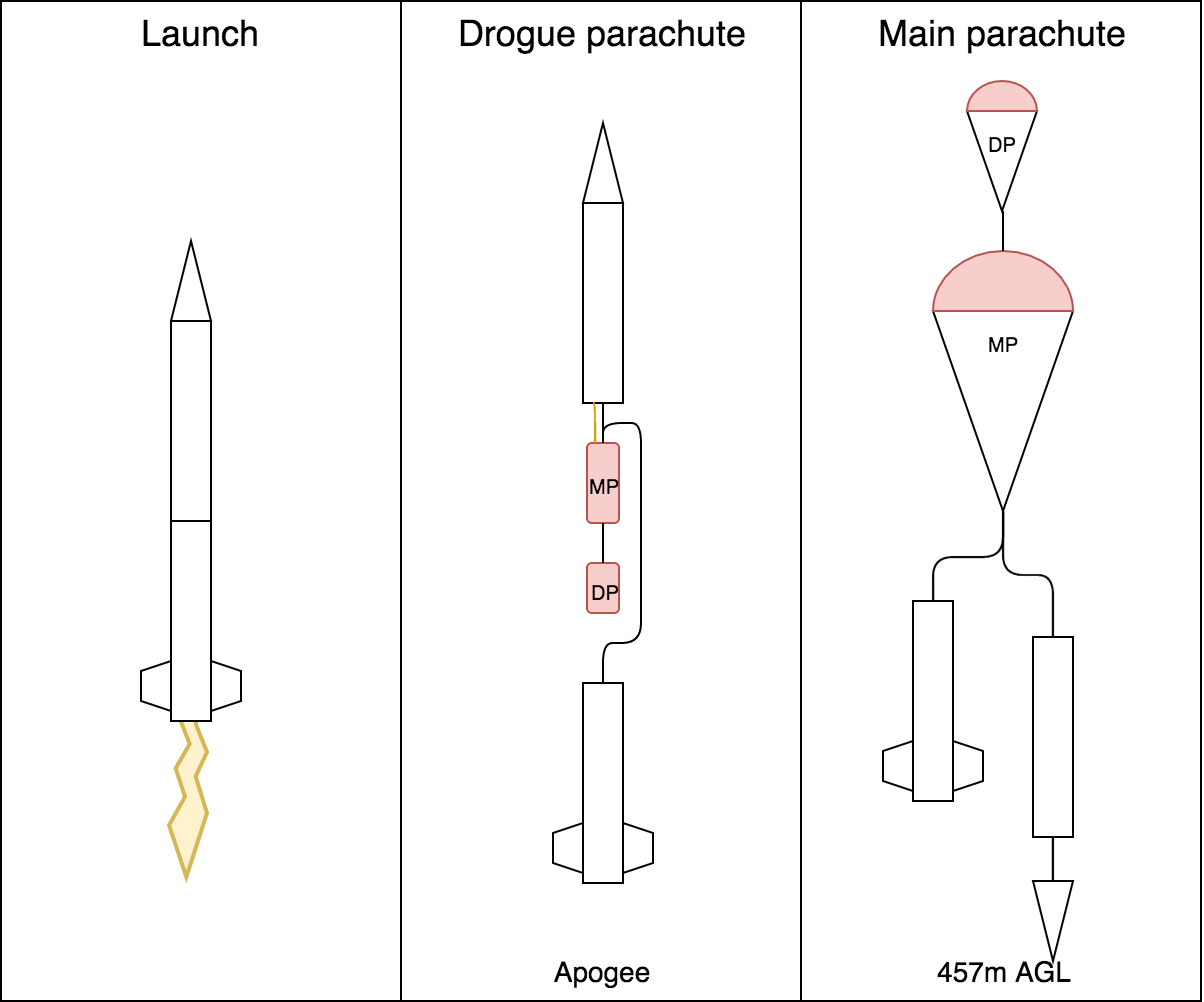
\includegraphics[width=0.3\textwidth]{img/recovery_conops_schema.png}
        \caption{Recovery Concept of Operations}
        \label{f:recovery_conops}
 \end{figure}

During the initial deployment the rocket is separated at the parachute bay and a drogue parachute is released to stabilize the attitude and reduce descent rate to 23-46m/s (75-150ft/s).At 457m AGL the main deployment takes place where the main parachute is released from the parachute bag to reduce the rocket's descent rate to less than 9m/s (30ft/s) to prevent excessive damage upon impact. Recovery Avionics system triggers the deployment events when the preprogrammed deployment conditions are met by firing a pyrotechnical charge.

\paragraph{Initial Deployment System}
The initial deployment is achieved by creating a pressure in the parachute bay and thus forcing the two rocket bodies to separate. The pressure is generated by puncturing a 23ml CO2 cartridge by a 0.2 ml black powder charge. The charge forces a puncture piston inside the cartridge seal to release the gas. This system is a COTS solution from Tinder Rocketry Recovery Solutions.
There are two redundant CO2 deployment systems each connected to two igniters. There are 2 redundant recovery electronic components in charge of triggering the system and each of the two can trigger both systems. Recovery avionics is outlined later in this section.

\paragraph{Main Deployment System}
The main parachute stowed in the parachute bag below the drogue parachute. The main parachute is held together by a wire which is cut at the programmed altitude. Then the load of the rocket pulls the main parachute out of the parachute bag. The setup is illustrated in Figure \ref{f:recovery_main_deployment}. The wire is cut by a shearing piston which is force through the wire by a 0.1ml black powder charge.Two wire cutters are installed for redundancy, one per recovery electronics.

\begin{figure}[h!]
 	\centering
        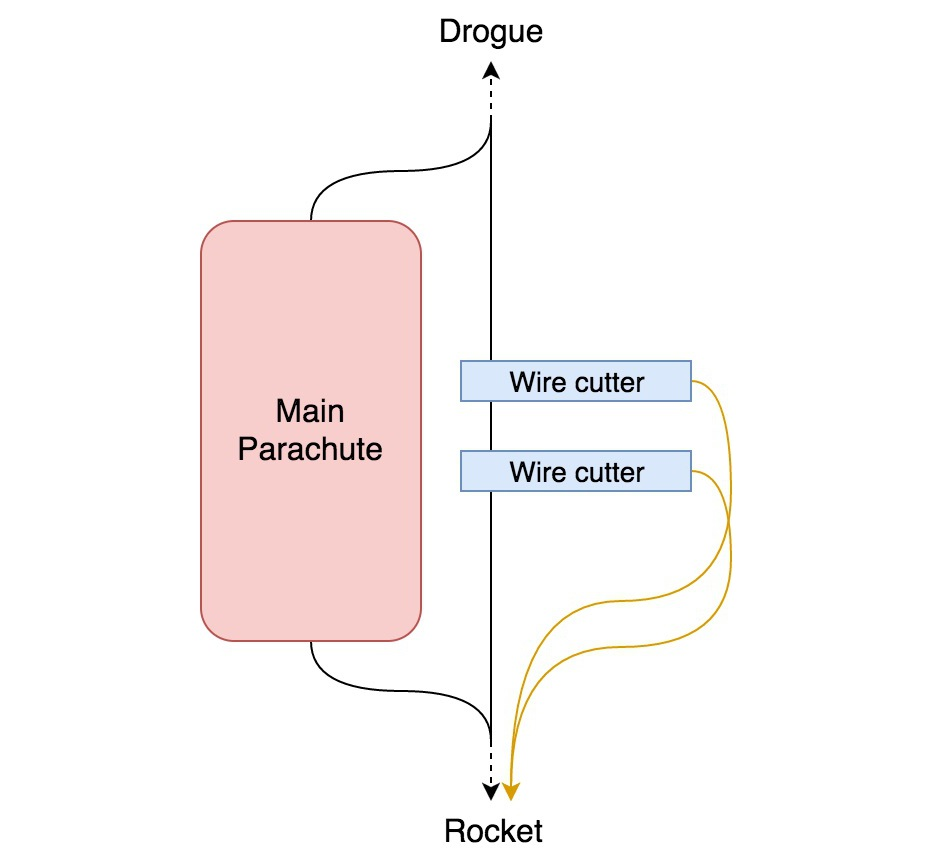
\includegraphics[width=0.3\textwidth]{img/recovery_main_deployment.jpg}
        \caption{Main Parachute Deployment}
        \label{f:recovery_main_deployment}
 \end{figure}
 
 \paragraph{Recovery Avionics}
The Recovery Avionics is designed for maximal reliability and features several levels of redundancy which is shown in Figure \ref{f:recovery_avionics_schema}. As required by the the competition rules we use two redundant electronics systems, which are two different COTS solutions.
The primary electronics is the AltimaxG3 from Rocketronics which features barometer and accelerometer sensors to estimate the altitude of the rocket. It uses a Kalman filter to estimate acceleration, speed and altitude of the rocket. This is more robust especially when pressure fluctuations can be expected at high velocity.
The backup electronics is the Raven3 from Featherweight Altimeters.
The primary electronics is programmed to detect the apogee and fire the two CO2 charges one after the other with a delay of 0.5 seconds. Then during descent it monitors air pressure until the main parachute deployment altitude is reached and deploys the wire cutter.
 The backup electronics is programmed as a timer to trigger the initial deployment after the predicted time to apogee from simulations. During descent it also detects the target altitude using a pressure sensor to trigger the main deployment
 
  \begin{figure}[h!]
 	\centering
        \includegraphics[width=0.5\textwidth]{img/recovery_avionics_schema.png}
        \caption{Recovery Avionics Schema}
        \label{f:recovery_avionics_schema}
 \end{figure}
 

\paragraph{Recovery Bay} 
 The recovery structure is made out of laser cut and milled plywood glued together with epoxy. It is screwed onto a circular bulkhead glued into the upper rocket tube. The connection to the parachute bay is made as airtight as possible by sealing holes with glue and using rubber washers.
Figure \ref{f:recovery_bay} shows the assembled recovery bay.
 \begin{figure}[h!]
 	\centering
        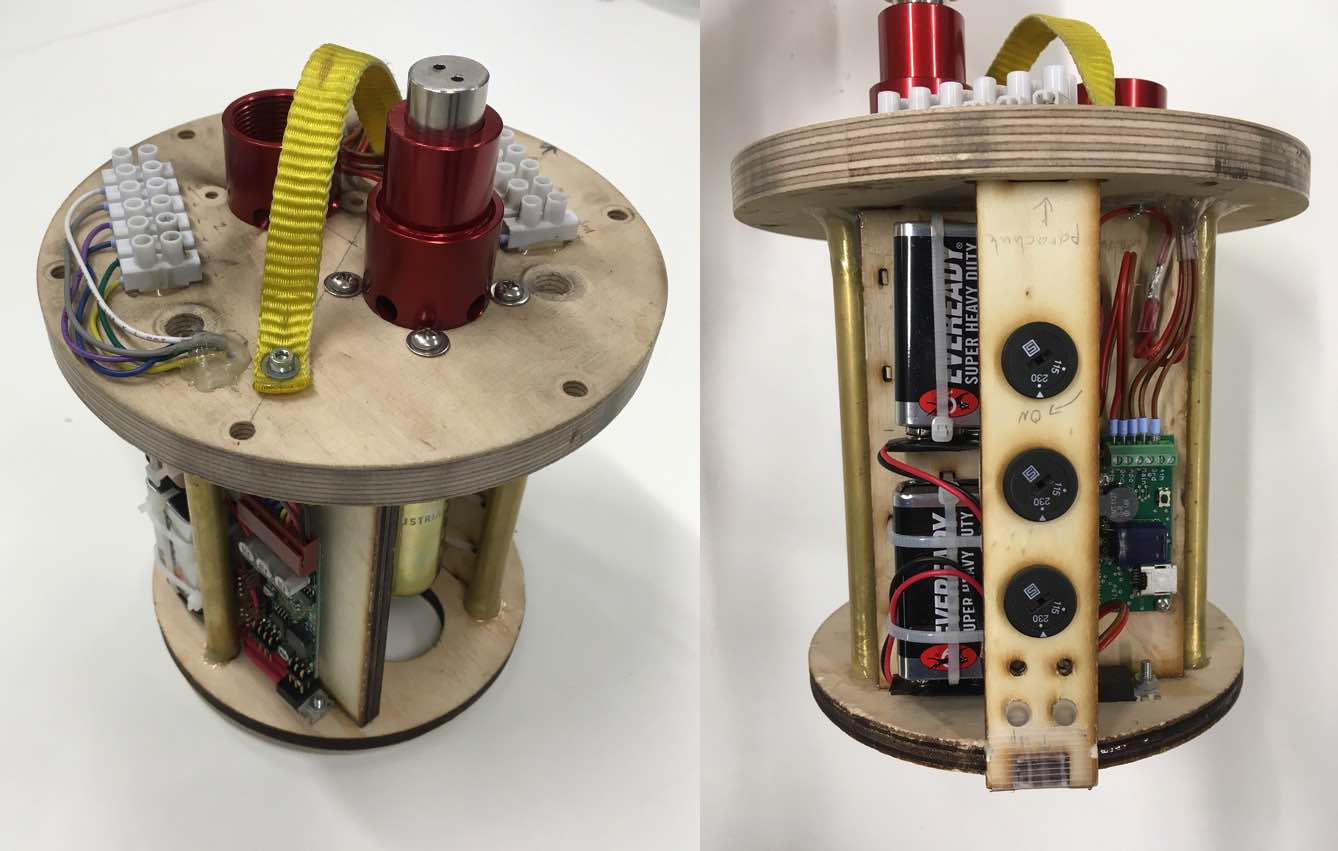
\includegraphics[width=0.3\textwidth]{img/recovery_bay.jpg}
        \caption{Recovery Bay}
        \label{f:recovery_bay}
 \end{figure}
 
 
\subsection{Avionics}
The avionics consist of 2 PCBs stacked together. The first one, referred to as the Interface Board (IB) shown in Figure \ref{f:avionics_ib}, is equipped with an absolute pressure sensor for altitude measurement, 2 differential pressure sensors for the Pitot tube, an IMU and a GNSS receiver. The IB also includes a XBee for telemetry downlink to the ground station, 64 MB of flash memory for data logging and 2 RS232 ports as well as an USB port. All these devices are controlled with an ARM microcontroller (STM32F4 of STMicroelectronics). The second PCB, the so called Power Board (PB) shown in Figure \ref{f:avionics_pb}, is equipped with a voltage regulator that power all the nosecone avionics and up to 6 servo outputs. All electronic components used for the avionics are automotive grade or better to ensure a proper working of the system under vibration and high temperature. Moreover, all the component were selected to be easily checked under microscope after soldering (e.g. no BGA chip are used as they usually require X-ray inspection).
The decision to split the avionics into 2 PCBs is made to overcome the limited space available and to avoid issues due to EMC.The buck converter on the PB can potentially generate a lot of EM perturbations, thus the sensitive parts such as the GNSS are placed away from it, namely on the IB.
As the rocket body is made of carbon fibre, the only RF transparent part of the rocket is the nosecone (made of fibre glass). Therefore, all the electronics components were integrated and placed there.

 \begin{figure}[h!]
 	\centering
        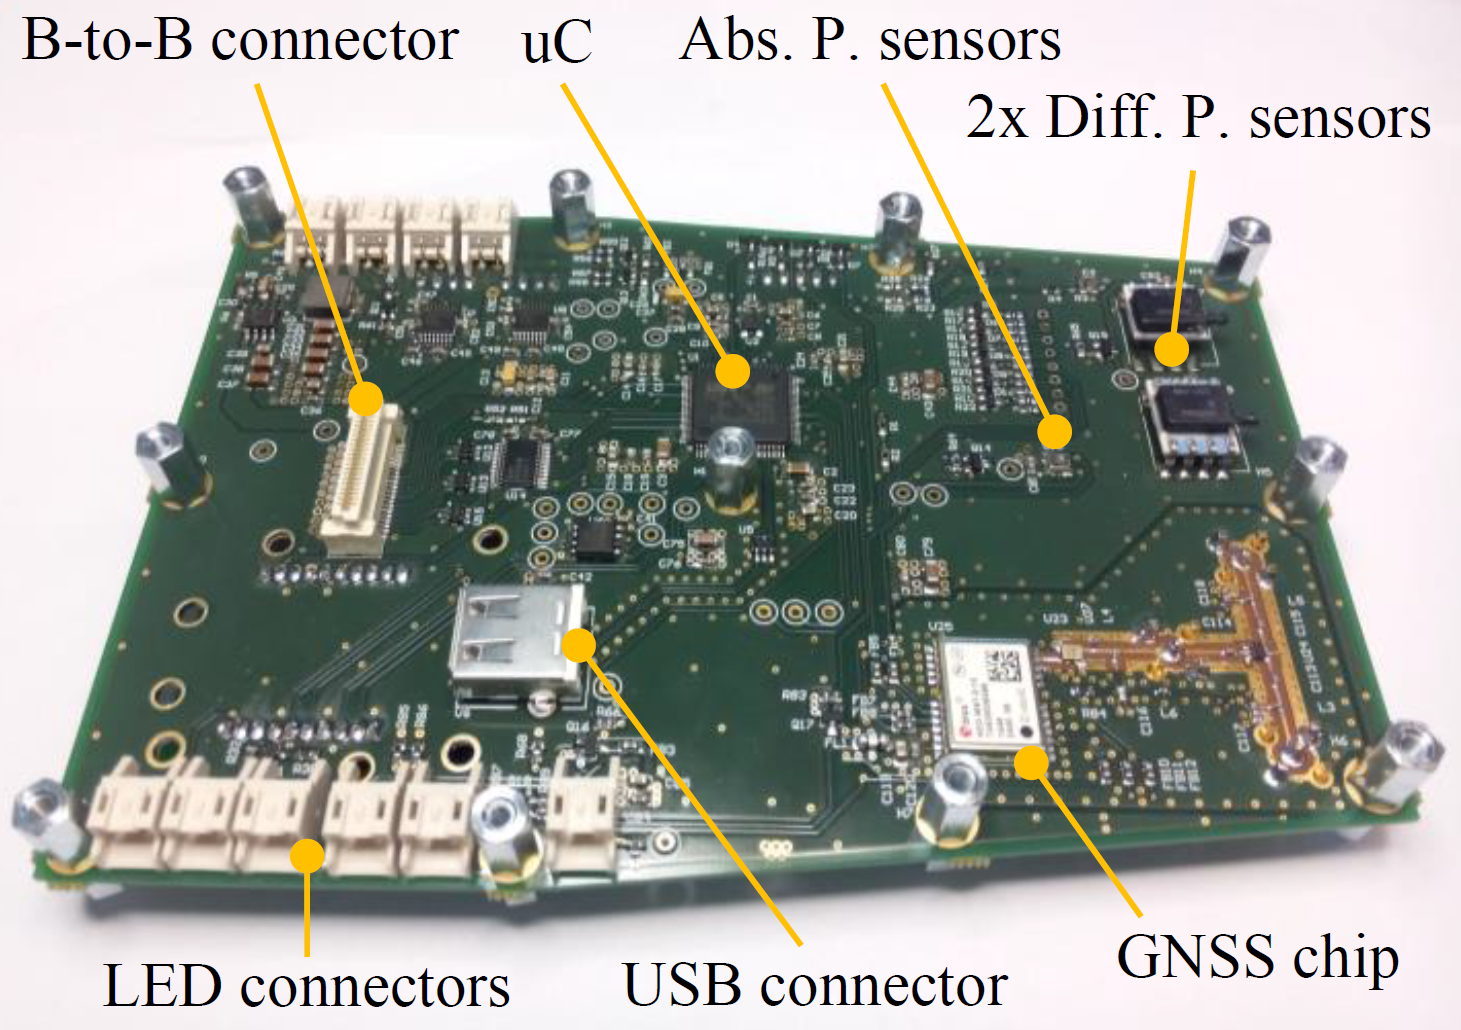
\includegraphics[width=0.20\textwidth]{img/AV_FIG_IB_top.PNG}
          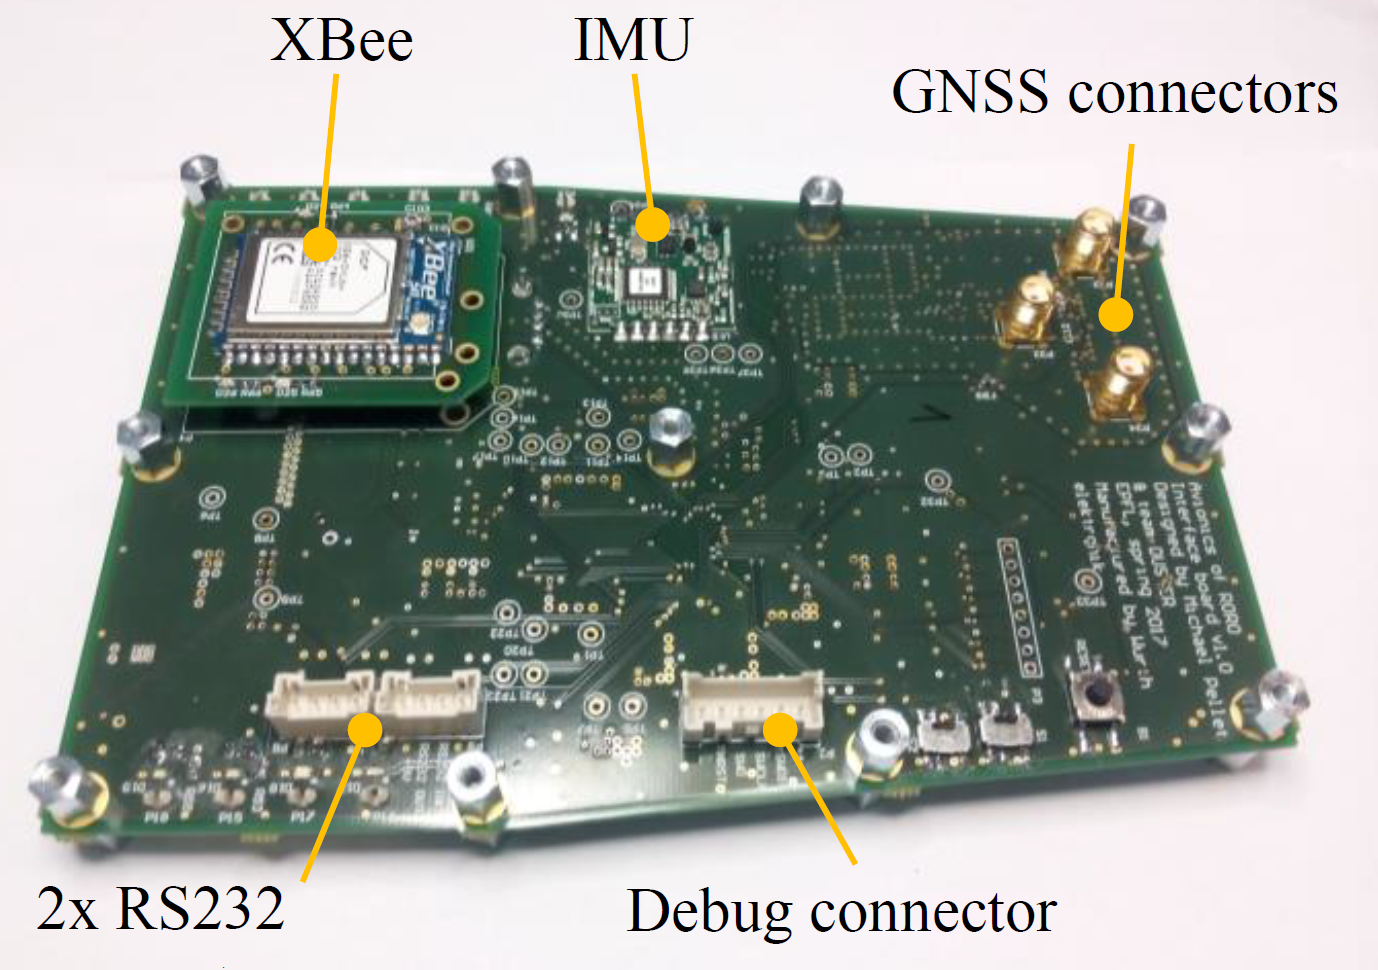
\includegraphics[width=0.20\textwidth]{img/AV_FIG_IB_bottom.PNG}
        \caption{Left: Interface Board (IB) Top, Right: Interface Board (IB) Bottom}
        \label{f:ib}
 \end{figure}
 
  \begin{figure}[h!]
 	\centering
        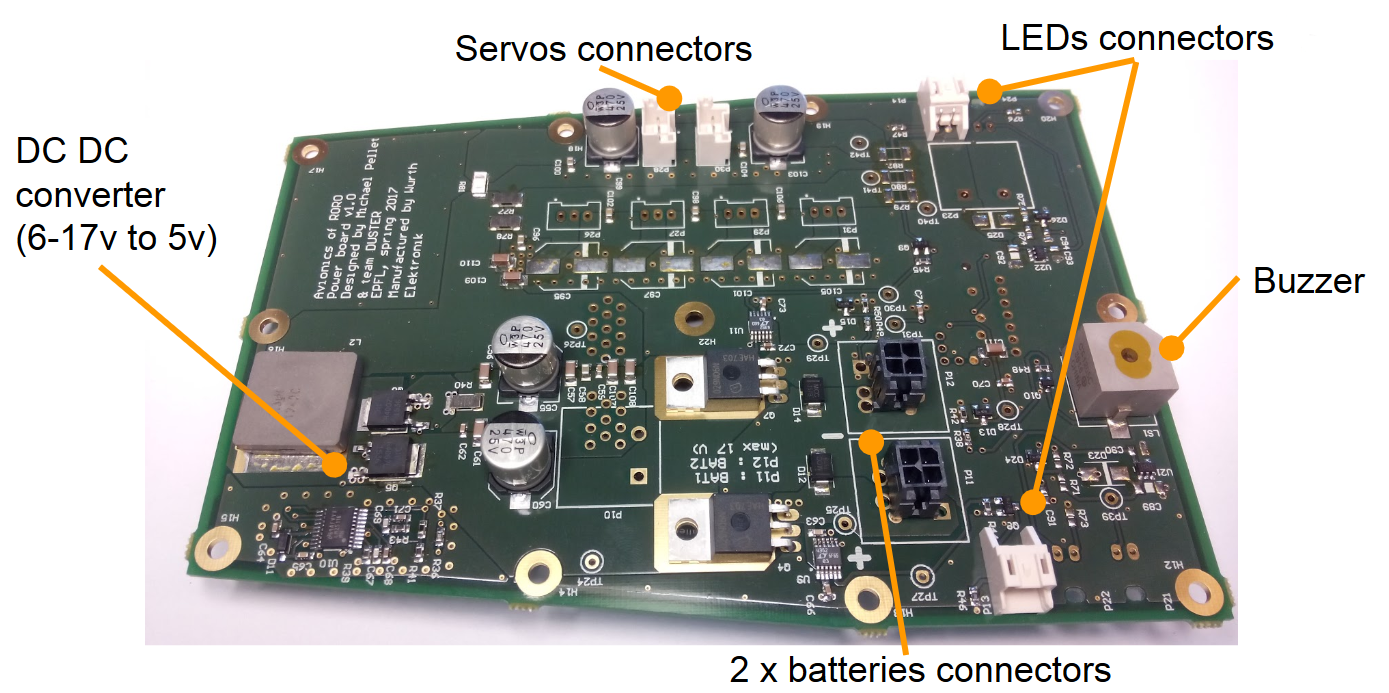
\includegraphics[width=0.20\textwidth]{img/AV_FIG_PB_top.PNG}
          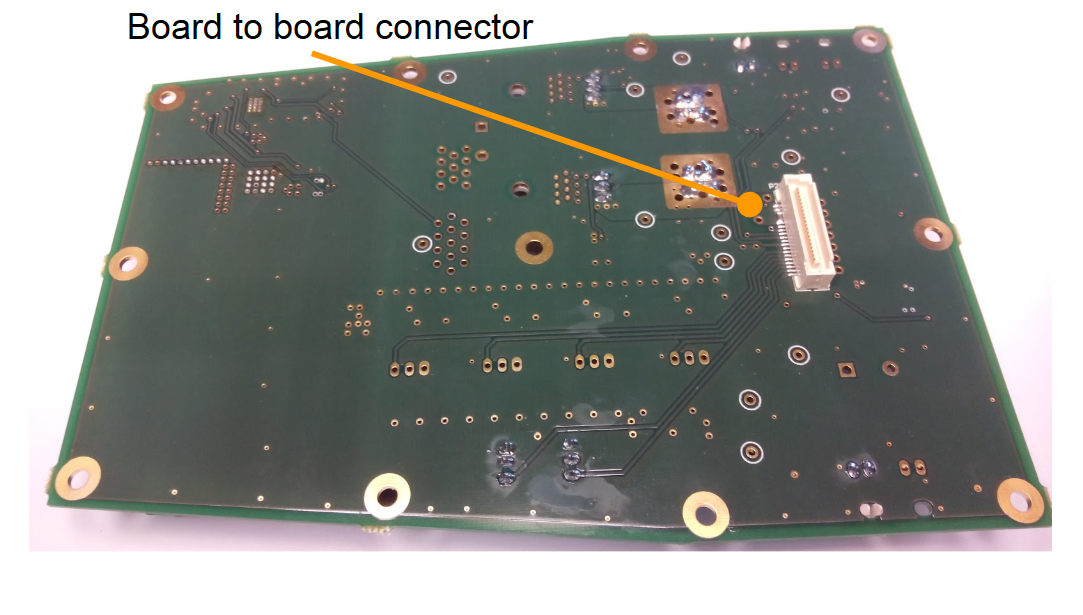
\includegraphics[width=0.20\textwidth]{img/AV_FIG_PB_bottom.PNG}
        \caption{Left: Power Board (PB) Top, Right: Power Board (PB) Bottom}
        \label{f:pb}
 \end{figure}

\paragraph{Sensors}
The Pitot tube uses 2 differential pressure sensors of Honeywell in parallel with different pressure range (0 to 6890Pa and 0 to 103350 Pa). This allows reduction of uncertainties at low speed (uncertainty of 6 m/s at 10m/s) and ensues good performances at higher speed (uncertainty of 2m/s at 280m/s). The IMU (3 Space High-G of Yost Labs) which is directly soldered on the IB can measure acceleration up to 24g and rate of turn up to 2000/s. Bu using its integrated data possessing unit, it can directly output orientation (Euler angles, quaternions or rotation matrix) as well as acceleration, rate of turn, magnetic field and velocity increments with a data rate of up to 250 Hz.
The GNSS chip is a NEO-M8T of uBlox equipped with a SAW (surface acoustic waves) filter. As the telemetry antenna (XBee) is close to the 1st GNSS antenna, 2nd SAW filter (SF1186G of muRata) is placed just before the RF input in order to ensure an optimum operation of the GNSS (e.g. avoid jamming due to the XBee frequencies).There are 2 GNSS active antennas. One is placed at the back of the nose cone and is oriented toward the back of the rocket and the other one is placed at the front of the nose cone and is oriented toward the front of the rocket. The 2 GNSS active antennas are controlled via an RF switch on the IB. The first GNSS antenna is used during ascend of the rocket while the second one is used during the descent, after the deployment of the drogue parachute and the nosecone ejection.

\paragraph{Telemetry Downlink}
For the telemetry downlink, a 900MHz XBee (XB9X-DMUS-001 of Digi International) is placed on the IB and connected to a 2.1dBi omni antenna. Second XBee is directly connected to the ground station which uses a high gain Yagi antenna (23dB) that is manually oriented towards the rocked during flight. This configuration ensures a good power margin (45dBm) above the sensitivity level of the receiver when at maximum theoretical distance (5 km). The XBee on the IB is fixed with 2 screws and is easily accessible and replaceable in order to replace it according to the country of operation (868 MHz for CH and 900 MHz for the US). Using XBee at 2.4GHz (which is legal for both CH and US) was not an option as they don?t have a sufficient communication range

\paragraph{Actuators}
The PB is equipped with 6 servo outputs, each allowing to control a high power servo such as HITEC XXXX. These outputs could be used in the future to implement an active control system of the rocket. In RORO I, 2 of these outputs are used. One is used to control the mechanism which ejects the nosecone while the other is used to control the release of the payload (the glider). 

\paragraph{Power Supply}
A high power buck converter from Texas Instrument is implemented on the PB. This device allows to power the avionics with 5 VDC with up to 15 A with 2S to 4S (6V to 17V) LiPo batteries. The PB is also equipped with 2 ideal diodes IC that allow to use 2 batteries in parallel for redundancy. In the case of RORO I, 2 3S, 1800 mAh LiPo are used. 

\paragraph{Software}
The software implemented in the avionics for RORO I mainly integrates the following functionalities: Data logging in the flash memory of the measurements performed by the sensors, detection of the launch of the rocket (with a threshold on the acceleration data from the IMU), sending the data of the GNSS (position) to the ground station via the XBee module, detection of the apogee of the rocket in order to open the nosecone 5 seconds after this event using a servo and switching to the 2nd GNSS antenna after the deployment of the nosecone. Five seconds after the deployment of the nosecone, second servo is trigged which allows the deployment of the payload.

\subsubsection{Mechanical Design and Manufacturing}
\paragraph{Mechanical Integration of the Avionics in the Nosecone}
The mechanical structure is designed with the idea of having the avionics easily accessible on the field. The 2 avionics PCBs are staked between 2 CNC machined plates of 3 mm tick plywood and fixed together with PCB spacers. On each plywood plate, gliding structures made out on plywood are glued. This assembly, called the avionic drawer (AD), can be easily slided into the avionic rack (AR) which is a structure made of several parts of CNC machined 6 mm tick plywood fixed to the control panel. To secure the AD, the aluminum GNSS ground plane of the 1st GNSS antenna is fixed on the top of it with nuts to two M5 threaded rods. These 2 threaded rods pass trough the avionic rack and are fixed to the control panel. On the control panel side, a hook is fixed at the end of each threated rod. These hooks are used to fix the rope that link the nosecone to the upper body bulkhead. The structure made of the control panel on which the AR together with the AD is fixed can be slided into the nosecone and be fixed with 6 M3 screws to a plywood crown glued with epoxy to the nosecone. The Avionics Bay inside the nosecone is depicted in Figure \ref{f:avionics_bay}

  \begin{figure}[h!]
 	\centering
        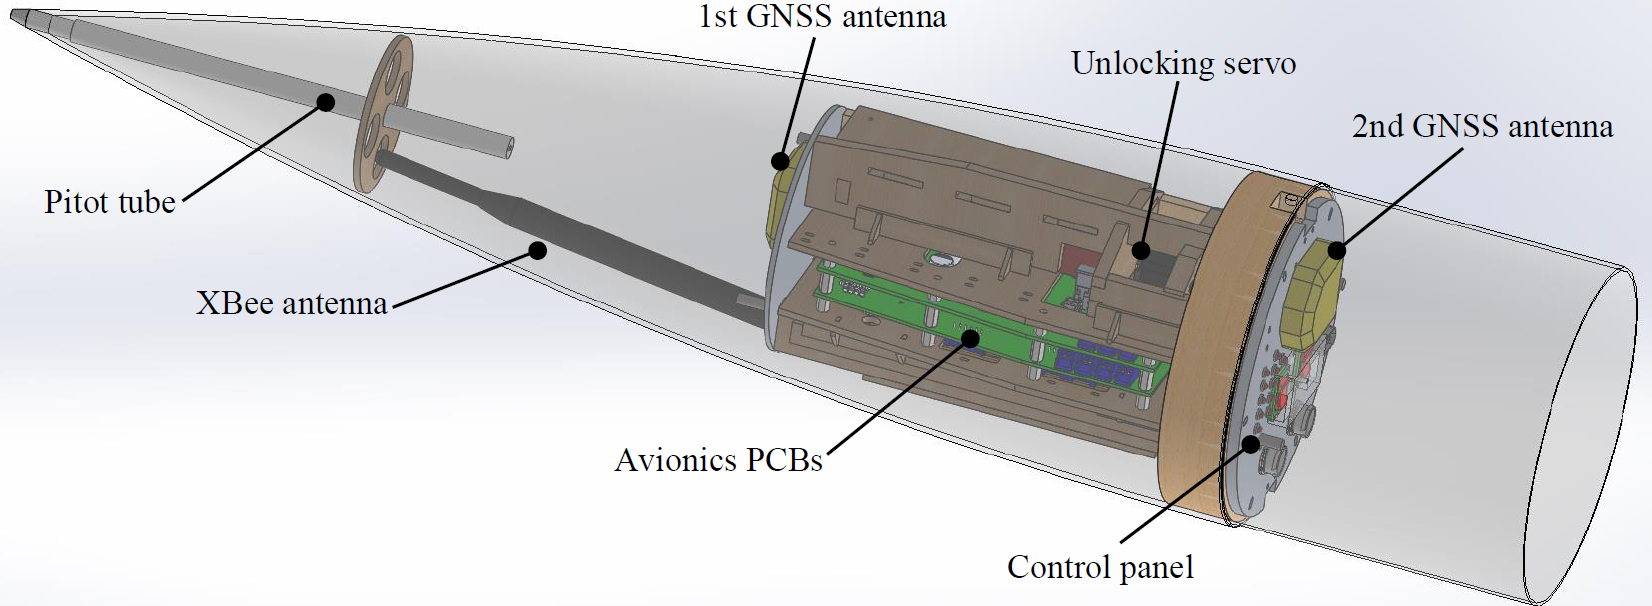
\includegraphics[width=0.45\textwidth]{img/AV_FIG_CAD_nosecone.PNG}
        \caption{Avionics Bay inside the Nosecone}
        \label{f:avionics_bay}
 \end{figure}
 
\paragraph{Pitot Tube}
The Pitot tube is made out of 3 fiberglass tube of in/out diameter: 2.5/4mm, 4/6mm and 6/8mm. These tubes are glued into each other with epoxy to form a tube of 2.5/8 mm diameter. At one end of this tube, a push-pull pneumatic adapter is glued. 5cm bellow the adapter a support made of LASER machined plywood is glued. The other end of the Pitot tube is glued with epoxy in a hole previously drilled at the tip of the nosecone and the plywood support is glued to the wall of the nosecone. Two holes are drilled on the side of the nosecone for the static pressure measurement.
A flexible pipe connected to the Pitot tube, is fixed on the wall of the nosecone and comes down to the control panel. From the control panel, a 2nd flexible pipe is fixed on the AD and goes to the 2 differential pressures sensors on the IB. A pneumatic push-pull connector allow to connect the 2 pipes together. When one needs to access the avionics bay, the pneumatic connector is removed as well as the 6 screws that fix the control panel to the nosecone and then, the control panel (that carries all the avionics) can be removed from the nosecone.

\paragraph{Nosecone Deployment System}
Note: in the following paragraph, everything noted in parenthesis refers to the Figure \ref{f:av_deployment_sys}
In order to get the satellite fix for the GNSS after apogee, the nosecone needs to be deployed. Moreover, this makes an opening in the upper body that allows to deploy the payload. So, to ensure the deployment of the nosecone, an ejection system was designed and manufactured that take into account the fact that the
main part of the volume bellow the nosecone is occupied by the payload.
The designed and manufactured system consist of 2 aluminum U-profiles (6.) fixed to the bulkhead (2.) of the upper body (1.). At the upper end of the u-profiles, a hook is fixed (7.) that is used by the looking system to secure the nosecone (5.). A gliding structure (3.) made out of 2 bigger aluminum U-profiles joined together with 4 arcs cut out of a phenolic tube can slide into the upper body.
In the smaller U-profiles (6.), a traction spring (4.) is fixed just bellow the hook (7.), the other end of the spring is fixed on the gliding structure (3.). So, when the nosecone is put in place, the upper part of the gliding structure comes in contact with the lower end of the nosecone and, thus, the gliding structure is pushed in the upper body which loads the 2 springs. When fully loaded, the 2 spring produce a total force of c.a. 100N. When the nosecone is released (thanks to the locking system) the gliding structure pushes it away from the upper body.

  \begin{figure}[h!]
 	\centering
        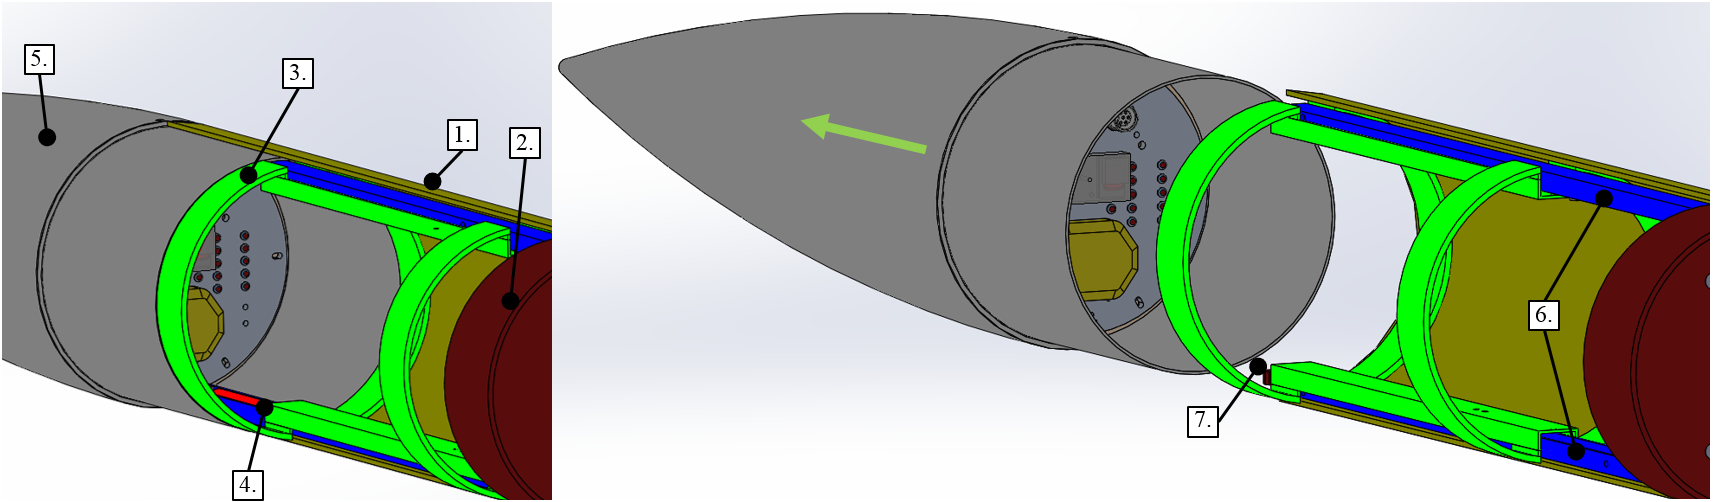
\includegraphics[width=0.45\textwidth]{img/AV_FIG_CAD_depl_sys_1.PNG}
        \caption{Deployment System of the Nosecone. Left: In place on the upper body. Right: after deployment. (for clarity, payload is not shown)}
        \label{f:av_deployment_sys}
 \end{figure}

\paragraph{Nosecone Locking System}
Note: in the following paragraph, everything noted in parenthesis refers to the Figure \ref{f:av_locking_sys}
To secure the nosecone in place during the ascend of the rocket, a locking system was designed and manufactured. This system consist out of 2 steel pins of 6 mm diameter (2. and 3.) loaded with a compressive spring (4.) that can slide in a structure (1.) fixed to the control panel of the nosecone. An ?inverted? came wheel (5.) controlled with a servo that is fixed to the AR is used to move the 2 pins forth and back. When locked, the end of the 2 pins goes in a hook (7.) fixed to each outer rail (6.) of the
deployment system. When unlocked, the steel rods are retracted and comes out of the hooks. 
This configuration, with an inverted came wheel, allows to unlock the nosecone from the outside even if there is a failure of the servo or the avionics. Indeed, the axis of the 2 locking steel rods is aligned with the 2 holes (8.) made in the nosecone for Pitot tube?s static pressure measurement, thus, the locking system can be unlocked using 2 screwdriver to push the pins inside the nosecone

  \begin{figure}[h!]
 	\centering
        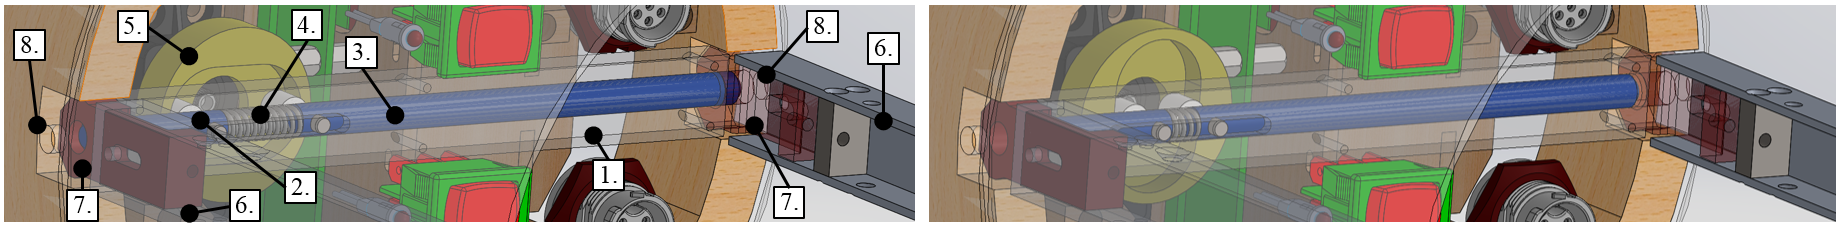
\includegraphics[width=0.45\textwidth]{img/AV_FIG_CAD_lockingsystem_2.PNG}
        \caption{Locking System of the Nosecone. Left: locked, Right: unlocked}
        \label{f:av_locking_sys}
 \end{figure}

\subsection{Flight Tests-PATRICK}
\label{subsection:flightTests}